\documentclass[tikz,svgnames]{standalone}

\usetikzlibrary{mindmap}

\begin{document}

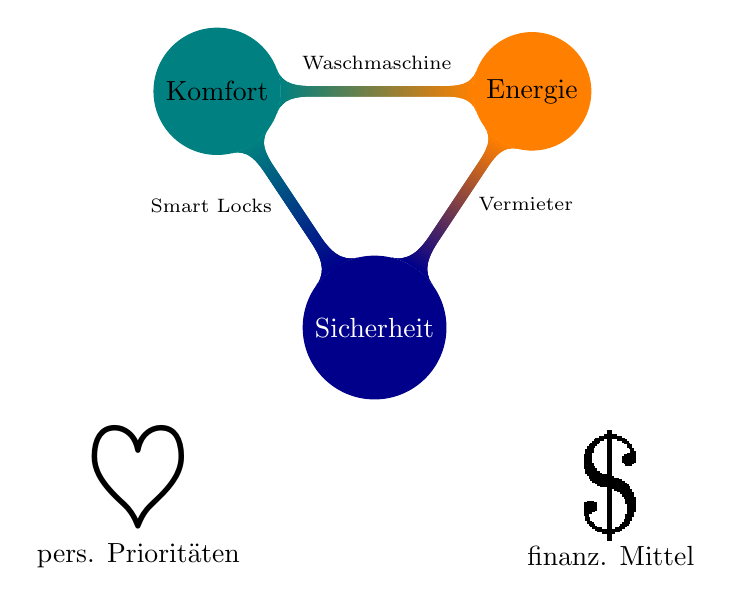
\begin{tikzpicture}

  \begin{scope}[concept color=orange]
    \node (Energie) at (2,0) [concept] {Energie};
  \end{scope}

  \begin{scope}[concept color=teal]
    \node (Komfort) at (-2,0) [concept] {Komfort};
  \end{scope}

  \begin{scope}[concept color=DarkBlue,text=white]
    \node (Sicherheit) at (0,-3) [concept] {Sicherheit};
  \end{scope}

  \path (Energie) to[circle connection bar switch color=from (orange) to (teal)] (Komfort);

  \path (Energie) to[circle connection bar switch color=from (orange) to (DarkBlue)] (Sicherheit);

  \path (Komfort) to[circle connection bar switch color=from (teal) to (DarkBlue)] (Sicherheit);

  \path (Energie) to[circle connection bar switch color=from (orange) to (teal)] node[above=1ex]{\scriptsize{Waschmaschine}} (Komfort);

  \path (Energie) to[circle connection bar switch color=from (orange) to (DarkBlue)] node[right=1ex]{\scriptsize{Vermieter}} (Sicherheit);

  \path (Komfort) to[circle connection bar switch color=from (teal) to (DarkBlue)] node[left=1ex]{\scriptsize{Smart Locks}} (Sicherheit);

  \node (Herz) at (-3,-5) {\scalebox{5}{$\heartsuit$}};
  \node (Herzschrift) at (-3,-5.9) {pers. Prioritäten};

  \node (Herz) at (3,-5) {\scalebox{5}{\$}};
  \node (Herz) at (3,-5.9) {finanz. Mittel};

\end{tikzpicture}

\end{document}